\documentclass[twoside,openany,12pt]{beautynote} 
% Input Some Information of the doc
\doctitle{Complex Geometry}
\docsubtitle{Logarithmic vanishing theorems on compact K\"ahler manifolds}
\dockeywords{Vanishing theorems, K\"ahler manifolds}
\date{\today\vfill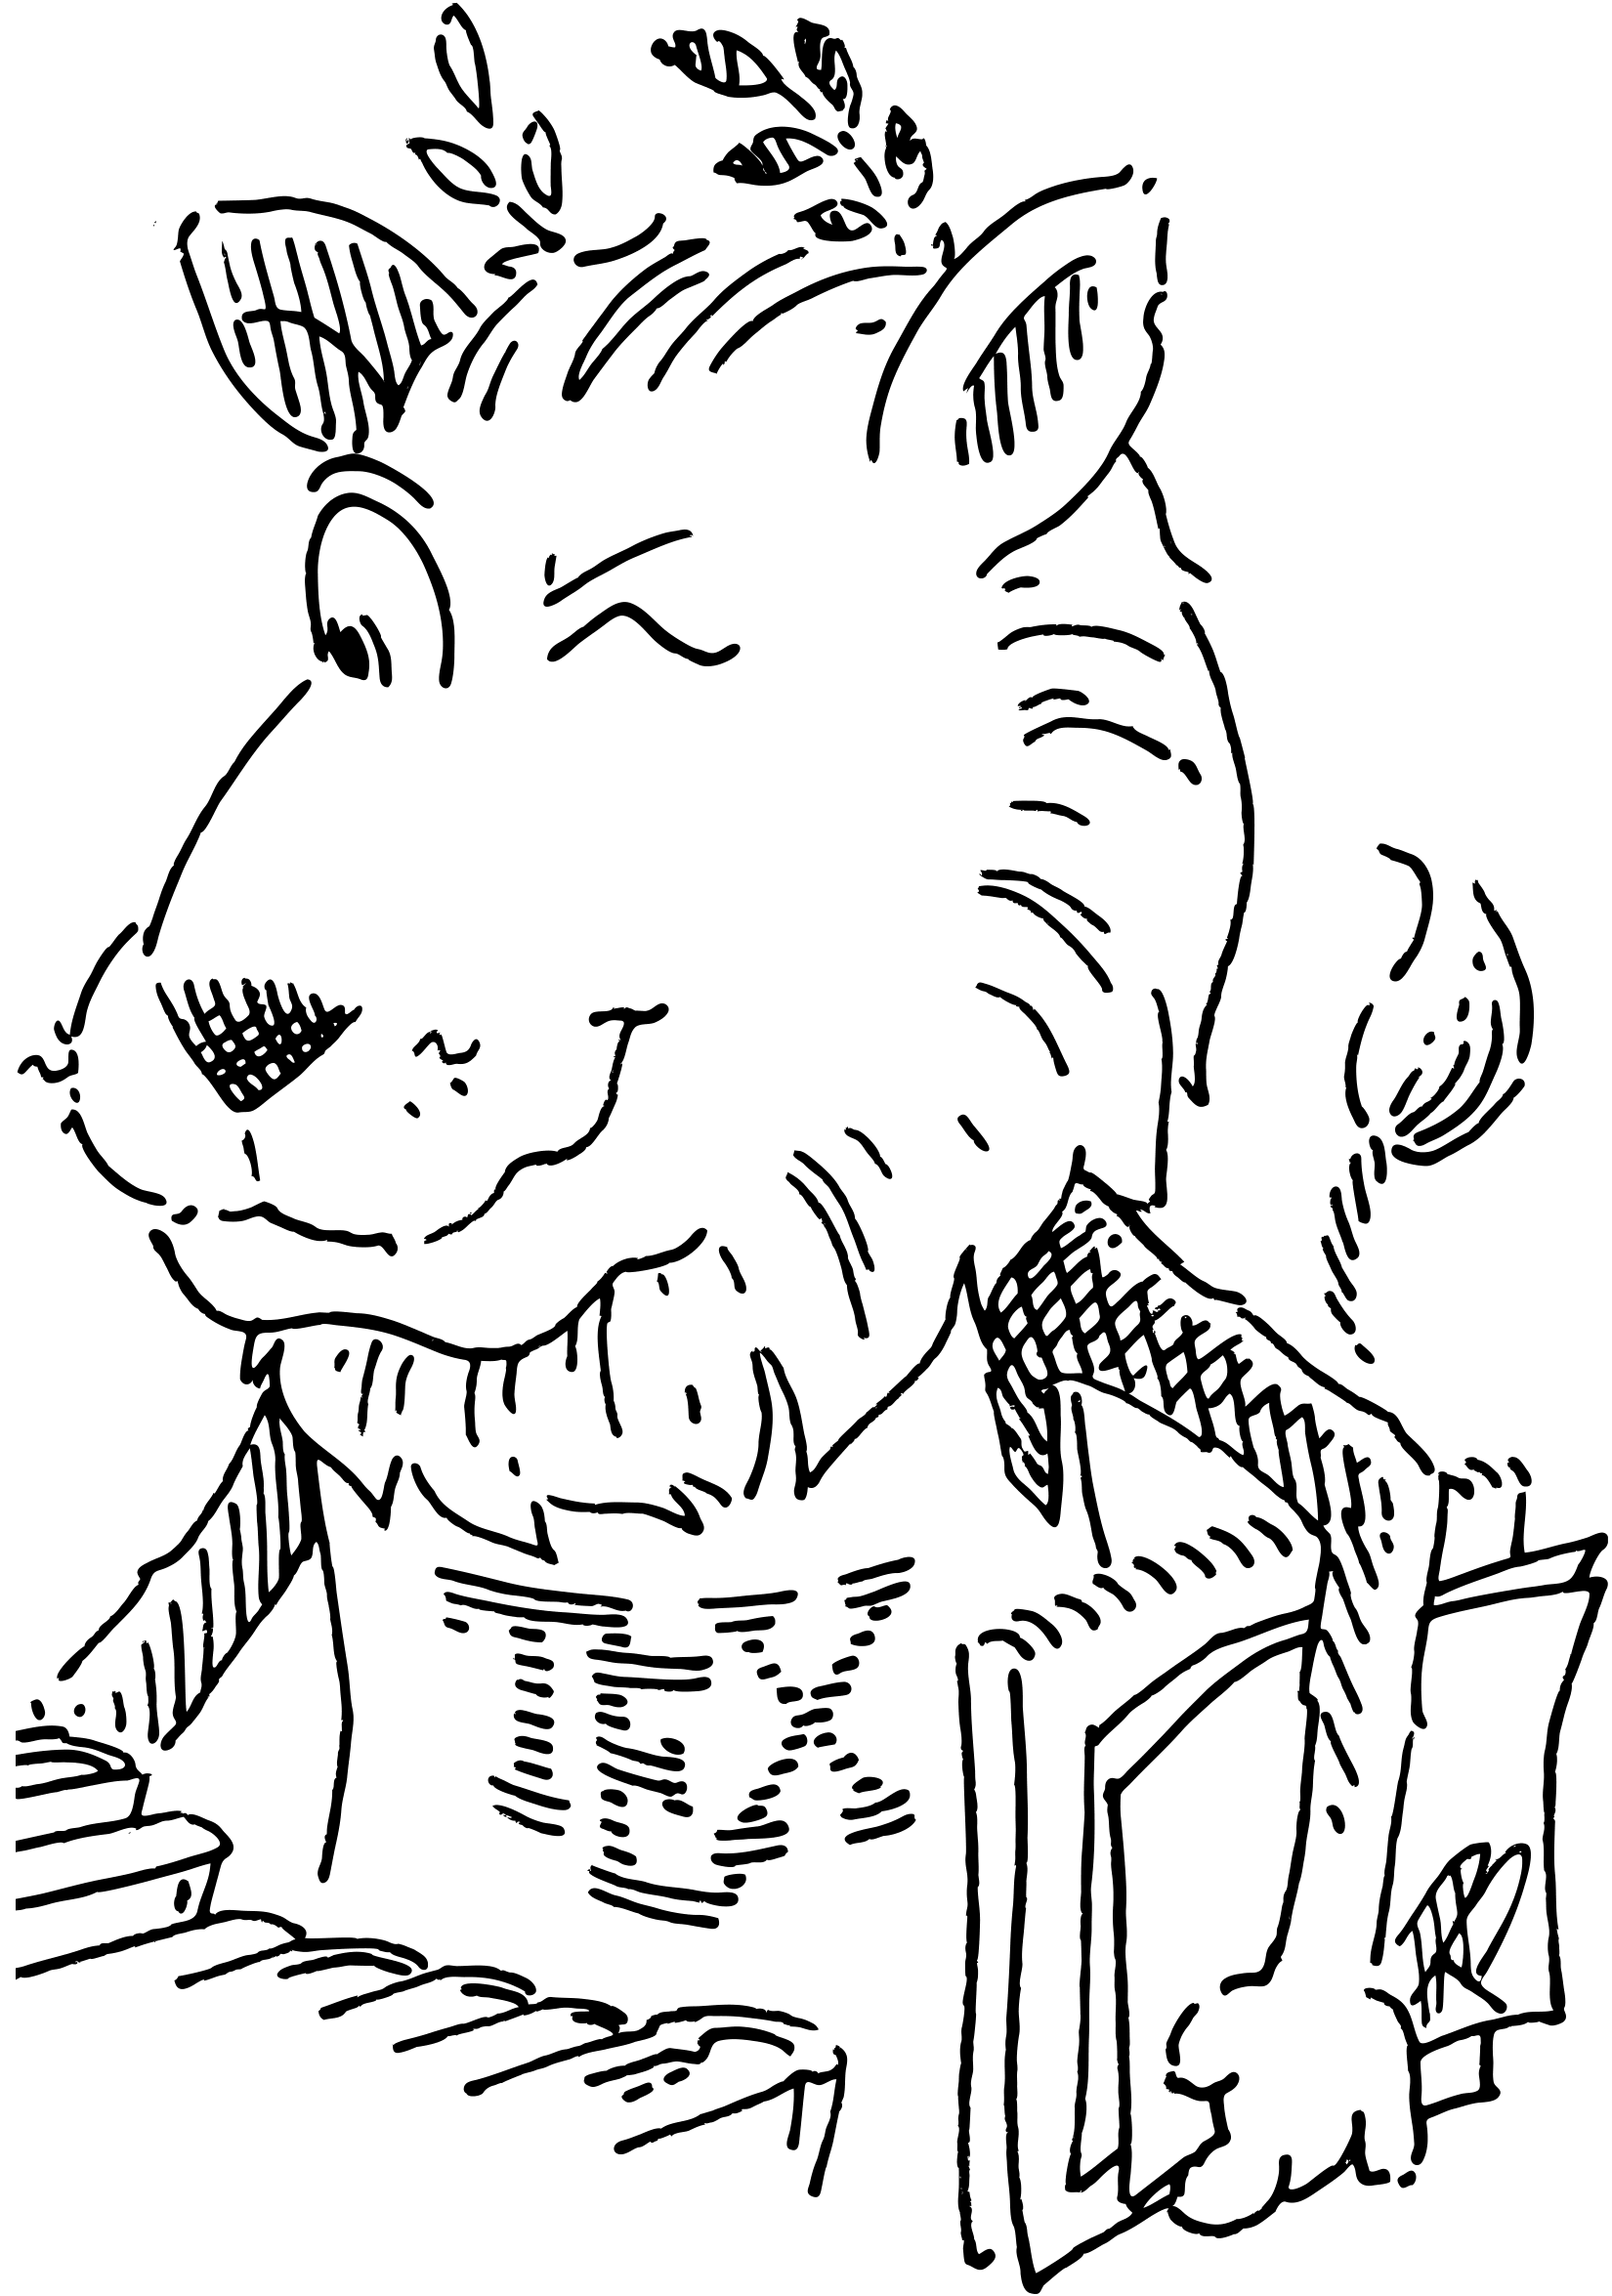
\includegraphics[width=0.15\textwidth]{titlepage.png}\\[.1em] \textsc{\large Beautynote}}
% Hyperref always required second to last.
\RequirePackage{hyperref}
\makeatletter
\hypersetup{%
    % hidelinks,
    pdfstartview=Fit,%
    pdfmenubar=true,%
    pdftoolbar=true,%
    bookmarksopen=false,%
    colorlinks=true,
    linkcolor=black,
    citecolor=purple,
    pdftitle={\@docsubtitle},%
    pdfauthor={\@author},%
    pdfsubject={\@doctitle},%
    pdflang={\languagename},%
    pdfkeywords={\@dockeywords},%
    pdfproducer={pdfTeX}}
\makeatother

% Cleveref as the last one.
\RequirePackage{cleveref}
%%%%%%%%%%%%%%%%%
\author{Ethan Lu}
\footext{}
\copyrightpage%
{Faculty of Pure Mathematics}% Your Faculty
{Sun Yat-Sen University}% Your University
{Press of Sun Yat-Sen University}% Your Publisher
{01A75, 00B50}% AMS
{Guang Zhou}% Your City
% If you do not want to fill one of the fields, please leave it like this: {}
\usepackage{appendix}
\usepackage{mathrsfs}
\usepackage{symbols}
\usepackage{bropd}
\usepackage{bm}
\usepackage{tabularray,booktabs}
\begin{document}
% Titlepage
\maketitle\clearpage
%%%%%%%%%%%%%%%% Copyright-Page %%%%%%%%%%%%%%%%%%%%%%%
\copyrights
\pagestyle{\auxsettings}
\makeatletter
\thispagestyle{copyright}
\ifdefempty{\@faculty}{}{\noindent{\large\textsc{\@faculty}} \\}
\ifdefempty{\@university}{}{{\large\textsc{\@university}} \\[1em]}
\ifdefempty{\@publisher}{}{\textit{Published by:} \@publisher \\}
\ifthenelse{\boolean{copyright}}{\textit{Copyright by:} \textsc{\templateauthor }\\}{} 
\ifdefempty{\@ams}{}{\textit{AMS Classification (2020):} \@ams.\\}
\vfill
\ifdefempty{\@city}{}{\noindent\@city, on \today\\}
\copyright\,\the\year\, \textsc{The Authors}
\doclicenseThis
\cleardoublepage
\makeatother
%%%%%%%%%%%%%%%% Copyright-Page %%%%%%%%%%%%%%%%%%%%%%%
% Toc
    \tableofcontents
% Main Contents
\pagestyle{\defaultsettings}
\chapter{Preliminaries}
\section{Proof of Theorem1.1}
%%%%%%%%%% Start TeXmacs macros
\newcommand{\tmop}[1]{\ensuremath{\operatorname{#1}}}
%%%%%%%%%% End TeXmacs macros
\begin{lemma}[3.3]
    \[ \langle \left[ \sqrt{- 1} \Theta (V, h^V), \Lambda_{\tilde{\omega}_P}
    \right] u, u \rangle \geqslant C | u |^2 . \]
\end{lemma}

\begin{proof}
    \[ \Omega^p_Y \otimes {\color[HTML]{B4005A}K_Y^{- 1}} = \Omega^p_Y \otimes
        {\color[HTML]{B4005A}\Omega^{- n}_Y} = \Omega_Y^{- (n - p)} =^a
        \bigoplus_{i_1, \cdots, i_{n - p}} (F_{i_1}^{- 1} \otimes \cdots \otimes
        F_{i_{n - p}}^{- 1}) . \]
    \begin{eqnarray*}
        \Omega^p_Y \otimes {\color[HTML]{B4005A}\Omega^{- n}_Y} & = & \Omega^p_Y
        \otimes ({\color[HTML]{B4005A}\Omega^{- p}_Y} \otimes \Omega_Y^{- (n -
        p)})\\
        & = & (\Omega_Y^p \otimes 1) \otimes ({\color[HTML]{B4005A}\Omega^{-
        p}_Y} \otimes \Omega_Y^{- (n - p)})\\
        & = & (\Omega_Y^p \otimes 1) \otimes ({\color[HTML]{B4005A}\Omega^{-
        p}_Y} \otimes 1) \otimes (1 \otimes \Omega_Y^{- (n - p)})\\
        & = & 1 \otimes \Omega_Y^{- (n - p)} = \Omega_Y^{- (n - p)} .
    \end{eqnarray*}
    \[ (\Omega_Y^p \otimes 1) \otimes ({\color[HTML]{B4005A}\Omega^{- p}_Y}
    \otimes 1) = \Omega_Y^p ({\color[HTML]{B4005A}\Omega_Y^{- p}}) \otimes 1
    = 1 (\tmop{trivial} \tmop{holomorphic} \tmop{cotangent} \tmop{bundle})
    \otimes 1. \]
    $^a$ For $(\tmop{TY}, \tilde{\omega}_P) = \bigoplus_{i = 1}^n (F_i,
    \omega_i)$ by using (2.1), then in local case (Fixed a local coordinate $(W
    ; z_1, \cdots, z_n)$), one has $F_i^{\ast} = F_i^{- 1}$(Dual line
    bundle)\cite[\S 2.2,p71]{huybrechts2005complex}. ($\Omega_Y$ is the dual
    of $\tmop{TY}$) The conclusion is clear through some easy computation.
    
    We have
    \[ 
        \sqrt{- 1} \Theta (V, h^V)  =  \sum_{i_1, \cdots, i_{n - p}} \sqrt{-
        1} \Theta [L |_Y \otimes  (F_{i_1}^{- 1} \otimes \cdots
        \otimes F_{i_{n - p}}^{- 1})]
    \]
    and
    \begin{align*}
    {\color[HTML]{B4005A}\sqrt{- 1} \Theta [L |_Y \otimes 
    (F_{i_1}^{- 1} \otimes \cdots \otimes F_{i_{n - p}}^{- 1})]} & =  \sum_i
    \sqrt{- 1} \partial \overline{\partial} \log (\omega_i)\\
    (3.12) & \geqslant  \alpha \tilde{\omega}_P - (n - p) C
    \tilde{\omega}_P\\
    (\tmop{if} \alpha > (n - p + 1) C) & >  C\tilde{\omega}_P
    {\color[HTML]{B4005A}> 0} ,
    \end{align*}
where we denote 
    $$\sqrt{- 1} \Theta [L |_Y \otimes 
(F_{i_1}^{- 1} \otimes \cdots \otimes F_{i_{n - p}}^{- 1})]=\sqrt{- 1} \Theta [L |_Y \otimes 
(F_{i_1}^{- 1} \otimes \cdots \otimes F_{i_{n - p}}^{- 1}), h_Y^L\otimes \omega_{i_1}^* \otimes\cdots\otimes\omega_{i_{n-p}}^*].
$$
    Thus, the curvature of each summand of $L |_Y \otimes  (F_{i_1}^{-
    1} \otimes \cdots \otimes F_{i_{n - p}}^{- 1})$ is strictly positive, i.e.
    \[{\color[HTML]{B4005A}\sqrt{- 1} \Theta [L |_Y \otimes (F_{i_1}^{- 1} \otimes \cdots \otimes F_{i_{n - p}}^{- 1})]> 0}.
    \]
    \begin{align*}
        \left\langle \left[ \sqrt{- 1} \Theta (V, h^V), \Lambda_{\widetilde{\omega}_P}\right] u, u \right\rangle & =  \left\langle \left[ \sum_{i_1, \cdots, i_{n - p}}\sqrt{- 1} \Theta [L |_Y \otimes  (F_{i_1}^{- 1} \otimes \cdots\otimes F_{i_{n - p}}^{- 1})], \Lambda_{\widetilde{\omega}_P} \right] u, u\right\rangle\\
        & \geqslant (q\cdot C-(n-n))|u|^2\geqslant C|u|^2. \text{($q\geqslant 1$)}
    \end{align*}
    And the proof of the assertion that of the metric $\widetilde{h}^{L }_Y$ is Nakano
    positive is on following.
    \begin{align*}
        \sum_{i_1, \cdots, i_{n - p}} \sqrt{- 1} \Theta [L |_Y \otimes 
        (F_{i_1}^{- 1} \otimes \cdots \otimes F_{i_{n - p}}^{- 1})] & =  \sum_{i,j, \alpha, \gamma} \sqrt{- 1} R_{i \bar{j} \alpha}^{\gamma} \tmop{dz}^i
        \wedge d \bar{z}^j \otimes e^{\alpha} \otimes e_{\gamma}  (\textrm{cf P.5} )\\
        (R_{i \bar{j} \alpha}^{\gamma} = h^{\gamma \bar{\beta}} R_{i \bar{j} \alpha\bar{\beta}} ) & =  \sum_{i, j, \alpha, \beta} \sqrt{- 1} h^{\gamma
        \bar{\beta}} R_{i \bar{j} \alpha \bar{\beta}}  \tmop{dz}^i \wedge d\bar{z}^j \otimes e^{\alpha} \otimes \bar{e}^{\beta}\\
        \tmop{dz}^i = \left( u^i \frac{\partial}{\partial z^i} \right) & = \sum_{i, j, \alpha, \beta} \sqrt{- 1} h^{\gamma \bar{\beta}} R_{i \bar{j}
        \alpha \bar{\beta}}   \left( u^i \frac{\partial}{\partial z^i} \right)\wedge \left( \bar{u}^j \frac{\partial}{\partial \bar{z}^j} \right) \otimes e^{\alpha} \otimes \bar{e}^{\beta}\\
        & =  \sum_{i, j, \alpha, \beta} \sqrt{- 1} h^{\gamma \bar{\beta}} R_{i\bar{j} \alpha \bar{\beta}}  u^{i \alpha} \bar{u}^{j \beta} \left( \frac{\partial}{\partial z^i} \otimes e^{\alpha} \right) \wedge \left( \frac{\partial}{\partial\bar{z}^j} \otimes \bar{e}^{\beta} \right)\\
        & >  \sum_{i_1, \cdots, i_{n - p}} C \widetilde{\omega}_P > 0
    \end{align*}
    As $h^{\gamma\bar{\beta}}>0$, then we have $\sum_{i, j, \alpha, \beta} \sqrt{- 1} h^{\gamma \bar{\beta}} R_{i
    \bar{j} \alpha \bar{\beta}}  u^{i \alpha} \bar{u}^{j \beta}>0$, which immediately shows that $$\sum_{i, j, \alpha, \beta} R_{i
    \bar{j} \alpha \bar{\beta}}  u^{i \alpha} \bar{u}^{j \beta}>0.$$ Thus $\widetilde{h}^{L }_Y$ is Nakano positive. 
\end{proof}

\begin{theorem}[Main theorem]\label{thm:1.1}
    Let
    \begin{center}
        \begin{tblr}{hline{1,Z} = {1pt,gray}, hline{2-Y}={0.5pt,dotted}, row{odd} = {},row{even} = {brown9},rows={m},  column{1}= {.2\linewidth,c},column{2}= {.65\linewidth},
    width=0.9\textwidth+2pt, colspec={X|[dotted]X},
    }
            $X$ & A compact K\"ahler manifold \\ 
            $D$ & A small normal crossing (SNC) divisor\\ 
            $N$ & A line bundle   \\ 
            $\Delta=\sum_{i=1}^{s}\alpha_i D_i$ & an $\mathbb{R}$-divisor with $\alpha_i\in [0,1]$ such that $N\otimes\mathcal{O}_X([\Delta])$ is a $k$-positive $\mathbb{R}$-line bundle \\
            $L$ & A nef line bundle \\
        \end{tblr}
    \end{center}

Then we have 
    \[
        H^q(X,\Omega_X^p(\log D)\otimes L\otimes N)=0, \text{ for any } p+q\geqslant n+k+1.
    \]
\end{theorem}

\clearpage
    \begin{proof}[Proof: (A small sketch)]
        The following computation is of (4.5).
        \begin{align*}
            &\sqrt{- 1} \Theta (\mathcal{F}, h_{\alpha, \varepsilon, \tau}^{\mathcal{F}})\\
            & =  \sqrt{- 1} \Theta (L \otimes F \otimes \mathcal{O}_X (- [\Delta]),
            h_{\alpha, \varepsilon, \tau}^{\mathcal{F}})\\
            & =  \sqrt{- 1} \partial \overline{\partial} \log (h_{\alpha, \varepsilon,
            \tau}^{\mathcal{F}})\\
            & =  \sqrt{- 1} \partial \overline{\partial} \log (h^L) + \sqrt{- 1}
            \partial \overline{\partial} \log (h^F) + \sqrt{- 1} \partial
            \overline{\partial} \log (h^{\Delta})^{- 1} + \sqrt{- 1} \partial
            \overline{\partial} \log \left( \prod_{i = 1}^s \| \sigma \|^{2
            \tau_i}_{D_i} (\log^2 (\varepsilon \| \sigma_i
            \|^2_{D_i}))^{\frac{\alpha}{2}}  \right)\\
            & =  \sqrt{- 1} \partial \overline{\partial} \log (h^L) + \sqrt{- 1}
            \partial \overline{\partial} \log (h^F) + \sqrt{- 1} \partial
            \overline{\partial} \log \left( \prod_{i = 1}^s h^{a_i}_{D_i} \right)^{- 1}
            + \sqrt{- 1} \partial \overline{\partial} \log \left( \prod_{i = 1}^s \|
            \sigma \|^{2 \tau_i}_{D_i} \right) \\
            &+ \sqrt{- 1} \partial \overline{\partial}
            \log \left( \prod_{i = 1}^s (\log^2 (\varepsilon \| \sigma_i
            \|^2_{D_i}))^{\frac{\alpha}{2}}  \right)\\
            & =  \sqrt{- 1} \partial \overline{\partial} \log (h^L) + \sqrt{- 1}
            \partial \overline{\partial} \log (h^F) - \sum_{i = 1}^s a_i \sqrt{- 1}
            \partial \overline{\partial} \log (h _{D_i})  + \sum_{i = 1}^s \tau_i
            \sqrt{- 1} \partial \overline{\partial} \log (\| \sigma \|^2_{D_i}) \\ &+
            \sum_{i = 1}^s \alpha \sqrt{- 1} \partial \overline{\partial} \log (\log 
            (\varepsilon \| \sigma_i \|^2_{D_i}))\\
            & =  \sqrt{- 1} \partial \overline{\partial} \log (h^L) + \sqrt{- 1}
            \partial \overline{\partial} \log (h^F) - \sum_{i = 1}^s a_i c_1  (D_i) +
            \sum_{i = 1}^s \tau_i \sqrt{- 1} \partial \overline{\partial} \log (h_{D_i})
            \\ &+ \sum_{i = 1}^s \alpha \sqrt{- 1} \partial \left( \frac{\overline{\partial}
            \log  (\varepsilon \| \sigma_i \|^2_{D_i})}{\log  (\varepsilon \| \sigma_i
            \|^2_{D_i})} \right)\\
            & =  \sqrt{- 1} \partial \overline{\partial} \log (h^L) + \sqrt{- 1}
            \partial \overline{\partial} \log (h^F) - \sum_{i = 1}^s a_i c_1  (D_i) +
            \sum_{i = 1}^s \tau_i c_1  (D_i) \\ &+ \sum_{i = 1}^s \alpha \sqrt{- 1} \left(
            \frac{\partial \overline{\partial} \log  (\| \sigma_i \|^2_{D_i}) \cdot \log
            (\varepsilon \| \sigma_i \|^2_{D_i}) - \overline{\partial} \log  (\|
            \sigma_i \|^2_{D_i}) \wedge \partial \log  (\| \sigma_i
            \|^2_{D_i})}{( \log  (\varepsilon \| \sigma_i \|^2_{D_i})^2}
            \right)\\
            & =  \sqrt{- 1} \Theta (L, h^L) + \sqrt{- 1} \Theta (F, h^F) + \sum_{i =
            1}^s (\tau_i - a_i) c_1  (D_i) + \sum_{i = 1}^s \left( \frac{\alpha \sqrt{-
            1} \partial \overline{\partial} \log  (\| \sigma_i \|^2_{D_i})}{\log 
            (\varepsilon \| \sigma_i \|^2_{D_i}) } \right) \\ &+ \sqrt{- 1} \sum_{i = 1}^s
            \left( \frac{\alpha \partial \log  (\| \sigma_i \|^2_{D_i}) \wedge
            \overline{\partial} \log  (\| \sigma_i \|^2_{D_i})}{( \log 
            (\varepsilon \| \sigma_i \|^2_{D_i})^2} \right)\\
            & =  \sqrt{- 1} \Theta (L, h^L) + \sqrt{-
            1} \Theta (F, h^F) + \sum_{i = 1}^s (\tau_i - a_i) c_1  (D_i) + \sum_{i =
            1}^s \left( \frac{\alpha c_1 (D_i)}{\log  (\varepsilon \| \sigma_i
            \|^2_{D_i}) } \right) \\ &+ \sqrt{- 1} \sum_{i = 1}^s \left( \frac{\alpha
            \partial \log  (\| \sigma_i \|^2_{D_i}) \wedge \overline{\partial} \log  (\|
            \sigma_i \|^2_{D_i})}{( \log  (\varepsilon \| \sigma_i
            \|^2_{D_i})^2} \right) .
          \end{align*}
          where $h_{D_i} = \| \sigma_i \|^2_{D_i} $.
          \clearpage
        
    \end{proof}
        \begin{remark}
            \begin{align*}
                \mathcal{O}_X([D])\otimes\mathcal{O}_X(-[\Delta]) &=\mathcal{O}_X(\sum_{i=1}^{s}[D_i])\otimes\mathcal{O}_X(-\sum_{i=1}^{s}a_i[D_i])\\ 
                (\text{Dual line bundle})&=\sum_{i=1}^{s}a_i \mathcal{O}_X([D_i])\otimes\mathcal{O}_X(-[D_i])\\ 
                &=\sum_{i=1}^{s}a_i \mathcal{O}_X(1). \text{ (trivial line bundle)}
            \end{align*}
                
        \end{remark}
    \begin{definition}[Poincar\'e Type Metric]\label{def:Poincare type metric}
        A metric $\omega_Y$ is of Poincar\'e Type along $D$ if for each local
        coordinate chart $(W ; z_1, \cdots, z_n)$ along $D$, the restriction $\omega
        |_{W_{1 / 2}^{\ast}} $ is equivalent to the usual Poincar\'e type
        metric $\omega_P$ defined by
        \[ \omega_P = \sqrt{- 1} \sum_{i = 1}^k \frac{\tmop{dz}_j \wedge d
        \overline{z_j}}{| z_j |^2 \cdot \log^2 | z_j |^2} + \sqrt{- 1} \sum_{j =
        k + 1}^n \tmop{dz}_j \wedge d \overline{z_j} . \]
        Where $W_{r}^{\ast}=Y\cap W=(\Delta_r^*)^{k}\times (\Delta_r)^{n-k}, r\in (0,\frac{1}{2}]$.
    \end{definition}

    \begin{theorem}[The key theorem for the proof of the main theorem]\label{thm:3.1}
        Let
        \begin{center}
            \begin{tblr}{hlines = {1pt,gray}, row{odd} = {gray9},rows={m},  column{1}= {.1\linewidth,c},column{2}= {.45\linewidth},hline{2,3}={0.5pt,dotted},
        row{even} = {brown9},width=0.6\textwidth+2pt, colspec={X|[dotted]X},
        }
        $(X,\omega)$ & A compact K\"ahler manifold of dimension $n$\\ 
        $D$ & A SNC divisor in X\\ 
        $\omega_P$ & A smooth K\"ahler metric on $Y=X-D$ which is Poincar\'e Type along $D$\\ 
    \end{tblr}
        \end{center}
    
    Then there exists a smooth Hermitian metric $h_Y^L$ on $L|_Y$ such that the sheaf $\Omega^p(\log D)\otimes\mO(L)$ over $X$ has a fine resolution given by the $L^2$ Dolbeault complex $(\Omega_{(2)}^{p,*}(X,L,\omega_P,h_Y^L),\overline{\partial})$.
    
    In other words, we have an \textbf{exact sequence of sheaf over $X$}
    \[0\to \Omega^p(\log D)\otimes\mO(L)\to \Omega_{(2)}^{p,*}(X,L,\omega_P,h_Y^L)\]
    such that $\Omega_{(2)}^{p,q}(X,L,\omega_P,h_Y^L)$ is a \textbf{fine sheaf} for any $0\leq p,q\leq n$. In particular,
    \begin{equation}\label{eq:3.2}
        H^q(X,\Omega^p(\log D)\otimes\mO(L))\cong H^{p,q}_{(2)}(Y,L,\omega_P,h_Y^L)\cong \bH_{(2)}^{p,q}(Y,L,\omega_P,h_Y^L).
    \end{equation}
    \textbf{Note:} The isomorphism holds up to equivalence of metrics, i.e. if $\widetilde{\omega}_P\sim \omega_P$ and $\widetilde{h}_Y^L\sim h_Y^L$, then
    \[
        \bH_{(2)}^{p,q}(Y,L,\omega_P,h_Y^L)\cong \bH_{(2)}^{p,q}(Y,L,\widetilde{\omega}_P,\widetilde{h}_Y^L).
    \]
    ! Replacing the line bundle with vector bundle is still valid.
    \end{theorem}

    \newcommand{\tmstrong}[1]{\textbf{#1}}
    \newcommand{\tmem}[1]{\emph{#1}}
    \begin{problem}[Why $\Omega^{p, q}_{(2)} (X, E)$ is a fine
        sheaf over $X$?]\label{prob:fine sheaf}
        In the paper \cite[\S 2.3, P7]{huang2016logarithmic}, the author asserts that if $u
        \in \Gamma (U, \Omega^{p, q}_{(2)} (X, E))$ and $f \in C^{\infty} (X)$, then
        $fu \in \Gamma (U, \Omega^{p, q}_{(2)} (X, E))$. This demonstrates the
        existence of a partition of unity in $\Omega^{p, q}_{(2)} (X, E)$.
        Subsequently, the author claims that $\Omega^{p, q}_{(2)} (X, E)$ is a fine
        sheaf over $X$.
    \end{problem}
    
    \begin{proof}
        The basis for this assertion lies in the properties of fine sheaves and the
        specific construction of $\Omega^{p, q}_{(2)} (X, E)$:
        \begin{enumerate}
            \item  {\tmstrong{Definition of a Fine Sheaf}}: {\tmem{A sheaf $\mathcal{F}$ is
        considered ``fine'' if it satisfies certain partition of unity properties.}}
        In this context, it means that for any open cover $\{U_i \}$ of the
        underlying topological space $X$, there exist smooth functions $\rho_i \in
        C^{\infty} (X)$ with specific properties:
        \begin{itemize}
            \item $0 \leq \rho_i \leq 1$ for all $i$.
            \item supp$(\rho_i) \subseteq U_i$ (the support of $\rho_i$ is contained
            in $U_i$). 
            \item $\sum \rho_i (x) = 1$ for all $x$ in $X$ (the sum of $\rho_i$ at
            each point $x$ is $1$).
        \end{itemize}
        {\tmem{These partition of unity functions $\rho_i$ are crucial for gluing
        together local sections of the sheaf to obtain global sections.}}
        \item {\tmstrong{Construction of}} $\Omega^{p, q}_{(2)} (X, E)$: This sheaf
        represents smooth differential forms of type $(p, q)$ with values in a
        vector bundle $E$ over the manifold $X$. {\tmem{Its construction involves
        defining local sections on coordinate patches and specifying how these
        sections transition between overlapping patches.}}
        \item {\tmstrong{Demonstrating Fine Sheaf Property}}: In Section 2.3 of the
        paper, the author asserts that if $u$ is a section in $\Omega^{p, q}_{(2)}
        (X, E)$ and $f$ is a smooth function on $X$, then the product $fu$ is also a
        section in $\Omega^{p, q}_{(2)} (X, E)$. {\tmem{This demonstrates
        compatibility with the fine sheaf property because it shows that you can use
        smooth functions (such as the $\rho_i$ functions from the partition of
        unity) to combine sections locally without leaving the sheaf $\Omega^{p,
        q}_{(2)} (X, E)$.}}
        
        {\it\tmstrong{Essentially, this step ensures that $\Omega^{p, q}_{(2)} (X, E)$
        is closed under multiplication by smooth functions, which is a crucial
        property for a sheaf to be fine.}}
        \end{enumerate}
    \end{proof}
    
    \begin{remark}
        In summary,{\tmem{ the assertion that $\Omega^{p, q}_{(2)} (X, E)$ is a fine
        sheaf is based on the construction of $\Omega^{p, q}_{(2)} (X, E)$ and the
        demonstration that it satisfies the necessary partition of unity property
        when sections are multiplied by smooth functions.}} This property is
        essential for many purposes in differential geometry and {\tmem{allows for
        the gluing of local sections to obtain global sections over a manifold
        $X$.}}
    \end{remark}
\begin{problem}
    \begin{enumerate}
        \item How to get (3.5)?
        \item How to obtain the Laurentz series representation of $\sigma_I(z)$ on $W_{1/2}^*$?
        \item Why $\sigma$ is $L^2$ integrable on $W_r^*$ iff $\beta_j>-\tau_j$ along $D_j$ by using polar coordinates and Fubini Theorem (Example 2.4)?
        \item Why $\sigma$ and $\nabla \sigma$ have only logarithimic pole and $\sigma$ is a section of $\Omega^p(\log D)\otimes\mO(L)$ on $W$?
    \end{enumerate}
\end{problem}
\begin{proof}[Solution]
    \begin{enumerate}
        \item 
        \item The Laurentz series equation for several variables is 
        \[
            f(z_1,\cdots,z_n)=\sum_{J=-\infty}^{\infty} a_J (z_1-z_{1_0})^{j_1} \cdots (z_n-z_{n_0})^{j_n},\quad R_1\leqslant |z_i-z_{i_0}|\leqslant R_2,
        \]
        where $J=(j_1,\cdots,j_n)$.  $f(z_1,\cdots,z_n)$ is single-valued analysis in the annulus centered at every point $z_{i_0}$. The coefficients are
        \[
            a_J=\frac{1}{(2\pi i)^n} \int_{\Omega_1}\cdots \int_{\Omega_n} \frac{f(z_1,\cdots,z_n)}{(z_1-z_{1_0})^{j_1+1} \cdots (z_n-z_{n_0})^{j_n+1}}\dd z_J,
        \]
        where $\dd z_J=\dd z_1\wedge\cdots \wedge\dd z_n$ and $\Omega_1,\cdots,\Omega_n$ are counter-clockwise closed curves surrounding the expansion point $(z_{1_0},\cdots,z_{n_0})$ in each variable, and the order of inegration can be interchanged.

        By using the above equation, for a fixed point $(0,\cdots,0)\in W_{1/2}^*=\Delta_{1/2}^{*t}\times \Delta_{1/2}^{n-t}$, we have 
        \begin{align*}
            \sigma_I(z)=\sum_{J=-\infty}^{\infty} a_J (z_1)^{j_1} \cdots (z_t)^{j_t}, \quad J=(j_1,\cdots,j_t),
        \end{align*}
            where $a_J=\sigma_{IJ}(z_{t+1},\cdots,z_n)$ is a holomorphic function on $\Delta_{1/2}^{n-t}$. Thus $\sigma_I(z)$ is bounded on $W_r^*\subset W_{1/2}^*$, i.e. there exists a positive constant $M$ such that $\abs{\sigma_I(z)}\leqslant M$.
        \item By using polar coordinates, we obtain that
        \begin{align*}
            &\|\sigma\|^2_{L^2(W_r^*)} \\
            &=\sum_{|I|=p}\int_{W_r^*} |e|^2_{h^L} \br{ |\sigma_I(z)|^2 \prod_{\nu=1}^b \log^2 |z_{i_{p\nu}}|^2 \prod_{i=1}^t |z_i|^{2\tau_i}(\log^2 |z_i|^2)^{\alpha/2} } \omega_P^n \\
            &\leqslant \sum_{|I|=p}\int_{W_r^*}  \br{ |\sigma_I(z)|^2 \prod_{\nu=1}^b \log^2 |z_{i_{p\nu}}|^2 \prod_{i=1}^t |z_i|^{2\tau_i}(\log^2 |z_i|^2)^{\alpha/2} } \omega_P^n \\
            &\leqslant\sum_{|I|=p} \br{\underbrace{\int_0^{2\pi}\cdots \int_0^{2\pi}}_{b+t}}\br{\underbrace{\int_{0}^{\frac 12}\cdots \int_{0}^{\frac 12}}_{b+t}}  \br{ |\sigma_I(z)|^2 \prod_{\nu=1}^b \log^2 r_{i_{p\nu}}^2 \prod_{i=1}^t r_i^{2\tau_i}(\log^2 r_i^2)^{\alpha/2} } \omega_P^n \;\dd \bm{\theta}\dd \bm{r} \\ 
            &=\sum_{|I|=p}|\sigma_I(z)|^2 \prod_{\nu=1}^b\br{ \int_0^{2\pi}\int_{0}^{\frac 12} \log^2 r_{i_{p\nu}}^2 \dd \theta_{i_{p\nu}}\dd r_{i_{p\nu}} }\cdot \prod_{i=1}^t\br{ \int_0^{2\pi}\int_{0}^{\frac 12} r_i^{2\tau_i}(\log^2 r_i^2)^{\alpha/2} \dd \theta_i\dd r_{i} } \omega_P^n \\
            &=\sum_{|I|=p}(2\pi)^{b+t}{\color{purple}|\sigma_I(z)|^2} \prod_{\nu=1}^b\br{ \int_{0}^{\frac 12} \log^2 r_{i_{p\nu}}^2 \dd r_{i_{p\nu}} }\cdot \prod_{i=1}^t\br{ \int_{0}^{\frac 12} r_i^{2\tau_i}(\log^2 r_i^2)^{\alpha/2} \dd r_i } {\color{purple}\omega_P^n}\\ 
            &=\sum_{|I|=p}(2\pi)^{b+t} 2^{2b+\alpha t}{\color{purple}|\sigma_I(z)|^2} \prod_{\nu=1}^b\br{ \int_{0}^{\frac 12} \log^2 r_{i_{p\nu}} \dd r_{i_{p\nu}} }\cdot \prod_{i=1}^t\br{ \int_{0}^{\frac 12} r_i^{2\tau_i}(\log r_i)^{\alpha} \dd r_i } {\color{purple}\omega_P^n}\\ 
            &\leqslant \sum_{|I|=p}(2\pi)^{b+t} 2^{2b+\alpha t} M^2  \br{\prod_{\nu=1}^b\br{ \int_{0}^{\frac 12} \log^2 r_{i_{p\nu}} \dd r_{i_{p\nu}} }\cdot \prod_{i=1}^t\br{ \int_{0}^{\frac 12} r_i^{2\tau_i}(\log r_i)^{\alpha} \dd r_i } } \br{\frac 12}^n\\ 
            &<+\infty \text{\quad (By using Example 2.4)}
        \end{align*}
            where $|e|^2_{h^L}\in [\frac 12,1]$ over $W$ by hypothesis and $r_i=|z_i|$, $\dd\bm{r}=\dd r_{i_{p1}}\wedge \cdots \wedge\dd r_{i_{pb}}\wedge \dd r_{1}\wedge \cdots \wedge \dd r_{t}, \dd\bm{\theta}=\dd \theta_{i_{p1}}\wedge \cdots \wedge\dd \theta_{i_{pb}}\wedge \dd \theta_{1}\wedge \cdots \wedge \dd \theta_{t}$ . $(r\leq \frac 12)$ Thus $\sigma$ is $L^2$ integrable on $W_r^*$ iff $\beta_j>-\tau_j$ along $D_j$.
            \clearpage
        \item \begin{align*}
            \nabla \sigma(z) &=\sum_{\abs{I}=p} \nabla \br{\sigma_I(z) \zeta_{i_1}\wedge\cdots\wedge\zeta_{i_p}\otimes e}\\ 
            &=\sum_{\abs{I}=p} \dd\sigma_I(z) \wedge\zeta_{i_1}\wedge\cdots\wedge\zeta_{i_p}\otimes e+\sum_{\abs{I}=p} \sigma_I(z) \wedge\zeta_{i_1}\wedge\cdots\wedge\zeta_{i_p}\otimes \dd e\\
            &+ \sum_{\nu=1}^p \br{\sum_{\abs{I}=p} \sigma_I(z) \zeta_{i_1}\wedge\cdots\wedge(\dd\zeta_{i_\nu})\wedge\cdots\wedge\zeta_{i_p}\otimes e}\\ 
            &=\sum_{\abs{I}=p} \dd\sigma_I(z) \wedge\zeta_{i_1}\wedge\cdots\wedge\zeta_{i_p}\otimes e
        \end{align*}
            ,where \begin{align*}
                \dd\sigma_I(z) &=\sum_{J=-\infty}^{\infty} \dd \br{ a_J (z_1)^{j_1} \cdots (z_t)^{j_t}}\\ 
                &=\sum_{J=-\infty}^{\infty} \dd \br{a_J } (z_1)^{j_1} \cdots (z_t)^{j_t}+\sum_{J=-\infty}^{\infty} a_J \dd \br{(z_1)^{j_1} \cdots (z_t)^{j_t}}\\ 
                &=\sum_{J=-\infty}^{\infty} \dd \br{\sigma_{IJ}(z_{t+1},\cdots,z_n)} (z_1)^{j_1} \cdots (z_t)^{j_t}+\sum_{J=-\infty}^{\infty} \sigma_{IJ}(z_{t+1},\cdots,z_n) \dd \br{(z_1)^{j_1} \cdots (z_t)^{j_t}}
            \end{align*}
            and 
            \begin{align*}
                \sigma_{IJ}(z_{t+1},\cdots,z_n) &=\frac{1}{(2\pi i)^{n-t}} \int_{W_{1/2}^*}\frac{\sigma_I(z_{t+1},\cdots,z_n)}{(z_{t+1}-z_{{t+1}_0})^{j_{t+1}+1} \cdots (z_n-z_{n_0})^{j_n+1}}\dd z_{t+1}\wedge\cdots\wedge\dd z_n.
            \end{align*}
                As $\sigma_{IJ}(z_{t+1},\cdots,z_n)$ is a holomorphic function on $\Delta_{1/2}^{n-t}$, thus it has only removable singularity, and so as to $\sigma_I(z)$, which shows that $\sigma$ and $\nabla\sigma$ have only logarihmic pole.
                

    \end{enumerate}
\end{proof}



% \appendix
\chapter{Additional Material}
\section{Definition of Nef line bundle}
\begin{definition}[Nef line bundle (Algebraic version)]\label{def:nef line bundle}
    More generally, a line bundle $L$ on a proper scheme $X$ over a field $k$ is said to be nef if it has nonnegative degree on every (closed irreducible) curve in $X$ (The degree of a line bundle $L$ on a proper curve $C$ over $k$ is the degree of the divisor $(s)$ of any nonzero rational section $s$ of $L$.) A line bundle may also be called an invertible sheaf.
\end{definition}

The term ``nef'' was introduced by Miles Reid as a replacement for the older terms ``arithmetically effective'' (Zariski 1962) and ``numerically effective'', as well as for the phrase ``numerically eventually free''. The older terms were misleading, in view of the examples below.

\textit{Every line bundle $L$ on a proper curve $C$ over $k$ which has a global section that is not identically zero has nonnegative degree.} As a result, a basepoint-free line bundle on a proper scheme $X$ over $k$ has nonnegative degree on every curve in $X$; that is, it is nef.  More generally, a line bundle $L$ is called semi-ample if some positive tensor power $L^{\otimes a}$ is basepoint-free. It follows that a semi-ample line bundle is nef. Semi-ample line bundles can be considered the main geometric source of nef line bundles, although the two concepts are not equivalent; see the examples below.

A Cartier divisor $D$ on a proper scheme $X$ over a field is said to be nef if the associated line bundle $O(D)$ is nef on $X$. Equivalently, $D$ is nef if the intersection number $D \cdot C$ is nonnegative for every curve $C$ in $X$.

To go back from line bundles to divisors, the first Chern class is the isomorphism from the Picard group of line bundles on a variety $X$ to the group of Cartier divisors modulo linear equivalence. Explicitly, the first Chern class $\mathrm{C}_1(\mathrm{~L})$ is the divisor $(s)$ of any nonzero rational section $s$ of $L$.

\subsection{The nef cone}

To work with inequalities, it is convenient to consider $\mathbf{R}$-divisors, meaning finite linear combinations of Cartier divisors with real coefficients. The $\mathbf{R}$-divisors modulo numerical equivalence form a real vector space $N^1(X)$ of finite dimension, the Néron-Severi group tensored with the real numbers.  (Explicitly: two $\mathbf{R}$-divisors are said to be numerically equivalent if they have the same intersection number with all curves in $X$.) An $\mathbf{R}$-divisor is called nef if it has nonnegative degree on every curve. The nef $\mathbf{R}$-divisors form a closed convex cone in $N^1(X)$, the nef cone $\operatorname{Nef}(X)$.

The cone of curves is defined to be the convex cone of linear combinations of curves with nonnegative real coefficients in the real vector space $N_1(X)$ of 1-cycles modulo numerical equivalence. The vector spaces $N^1(X)$ and $N_1(X)$ are dual to each other by the intersection pairing, and the nef cone is (by definition) the dual cone of the cone of curves.

A significant problem in algebraic geometry is to analyze which line bundles are ample, since that amounts to describing the different ways a variety can be embedded into projective space. One answer is Kleiman's criterion (1966): for a projective scheme $X$ over a field, a line bundle (or $\mathbf{R}$-divisor) is ample if and only if its class in $N^1(X)$ lies in the interior of the nef cone.  (An $\mathbf{R}$-divisor is called ample if it can be written as a positive linear combination of ample Cartier divisors.) It follows from Kleiman's criterion that, for $X$ projective, every nef $\mathbf{R}$-divisor on $X$ is a limit of ample $\mathbf{R}$-divisors in $\mathrm{N}^1(\mathrm{X})$. Indeed, for $D$ nef and $A$ ample, $D+c A$ is ample for all real numbers $c>0$.

\begin{definition}[Metric definition of nef line bundles (Geometry version)]\label{def:Metric definition of nef line bundles}
Let $X$ be a compact complex manifold with a fixed Hermitian metric, viewed as a positive $(1,1)$-form $\omega$. Following Jean-Pierre Demailly, Thomas Peternell and Michael Schneider, \textbf{\color{purple} a holomorphic line bundle $L$ on $X$ is said to be nef if for every $\varepsilon>0$ there is a smooth Hermitian metric $h_\varepsilon$ on $L$ whose curvature satisfies $\Theta_h(L) \geqslant-\varepsilon \omega$.} When $X$ is projective over $C$, this is equivalent to the previous definition (that $L$ has nonnegative degree on all curves in $X$) which explains the more complicated definition just given. 
\end{definition}
    \begin{definition}[Logarithmic pole]\label{def:logarithmic pole}
        For a complex function $f(z)$, if there exists a pole at $z_0$ with the following form:
        \[\color{purple} f(z)\sim \frac{C}{(z-z_0)\log (z-z_0)},\]
        where $\sim$ denotes that the ratio tends to $1$ as $z\to z_0$, $C$ is a nonzero complex number, and $\log(z-z_0)$ represents the logarithmic function, then $z_0$ is called a logarithmic pole of the function $f(z)$.

        Note that the characteristic of a logarithmic pole is that the function becomes very large in magnitude as we approach points near $z_0$.
    \end{definition}



\section{Some computation}

\begin{align*}
    &e (\eta) [\tmop{ie} (\partial \bar{\partial} \varphi), \Lambda] + e
    (\bar{\partial} \eta) \bar{\partial}^{\ast}_{\varphi} - e (\bar{\partial}
    \eta)^{\ast} \bar{\partial} - e (\partial \eta) \partial^{\ast} + e
    (\partial \eta)^{\ast} \partial_{\varphi} \\
    &= e (\eta) [\tmop{ie} (\partial \bar{\partial} \varphi), \Lambda] +
    \bar{\partial} e (\eta) \bar{\partial}^{\ast}_{\varphi} -
    \bar{\partial}^{\ast} e (\eta)  \bar{\partial} - \partial e (\eta)
    \partial^{\ast} + \partial^{\ast} e (\eta)  \partial_{\varphi} \\
    &= e (\eta) {\color[HTML]{008080}[\tmop{ie} (\partial \bar{\partial}
    \varphi), \Lambda]} + e (\eta) \left[ {\color[HTML]{800080}\bar{\partial}
    \bar{\partial}^{\ast}_{\varphi}} - {\bar{\partial}^{\ast}}  \bar{\partial} -
    \partial \partial^{\ast} + \partial^{\ast} \partial_{\varphi} \right]
    \\
    &= e (\eta) [{\color[HTML]{008080}\bar{\partial}
    \bar{\partial}^{\ast}_{\varphi} +}
    {\color[HTML]{008080}\bar{\partial}^{\ast}_{\varphi} \bar{\partial} -
    \partial_{\varphi} \partial^{\ast} - \partial^{\ast} \partial_{\varphi}}] +
    e (\eta) \left[ {\color[HTML]{800080}\bar{\partial}
    \bar{\partial}^{\ast}_{\varphi}} - {\bar{\partial}^{\ast}}  \bar{\partial} -
    \partial \partial^{\ast} + \partial^{\ast} \partial_{\varphi} \right]
    \\
    &= \ldots + e (\eta) \left[ {\color[HTML]{800080}\bar{\partial} (- \bar{\ast}
    (\bar{\partial} - e (\bar{\partial} \varphi)) \bar{\ast})} -
    {\bar{\partial}^{\ast}}  \bar{\partial} - \partial \partial^{\ast} +
    \partial^{\ast}  (\partial - e (\partial \varphi)) \right] \\
    &= \cdots + e (\eta) \cdot - \bar{\ast} \left[
    {\color[HTML]{800080}\bar{\partial} ( \bar{\partial} - e (\bar{\partial}
    \varphi))} - {\bar{\partial} }  \bar{\partial} - \partial \partial  +
    \partial   (\partial - e (\partial \varphi)) \right] \bar{\ast} \\
    &= \cdots - e (\eta) \cdot - \bar{\ast} [{\color[HTML]{800080}\bar{\partial}
    e (\bar{\partial} \varphi)} + \partial  e (\partial \varphi)] \bar{\ast}  \\
    &= \cdots - e (\eta) \cdot e (\varphi) - \bar{\ast}
    [{\color[HTML]{800080}\bar{\partial} \bar{\partial} } + \partial  \partial]
    \bar{\ast} \\
    &= 0 ? 
  \end{align*}
  
  \begin{align*}
    &\bar{\partial} e (\eta) \bar{\partial}^{\ast}_{\varphi} +
    \bar{\partial}^{\ast}_{\varphi} e (\eta) \bar{\partial} - \partial_{\varphi}
    e (\eta) \partial^{\ast} - \partial^{\ast} e (\eta) \partial_{\varphi}
    \\
    &= e (\eta) [{\color[HTML]{008080}\bar{\partial}
    \bar{\partial}^{\ast}_{\varphi} +}
    {\color[HTML]{008080}\bar{\partial}^{\ast}_{\varphi} \bar{\partial} -
    \partial_{\varphi} \partial^{\ast} - \partial^{\ast} \partial_{\varphi}}]  \\
    &= \ldots 
  \end{align*}


% Bibliography
\clearpage
\pagestyle{\auxsettings}
\printbibliography[heading=bibintoc]
\end{document} 